%\chapter{USSS toolkits}
%shown in figure~\ref{fig:artificialnatural}
%pages~\pageref{tab:opposites1}
%and form (section~\ref{section:form}, page~\pageref{section:form}).

\chapter{Electronic Music 1}
\label{history1}

\section{Tools and people that saw the beginning of `the electric'}

In 1877, Thomas Alva Edison (1847-1931) invented the phonograph (from Greek: sound writer), a hollow cylinder engraved with a spiral groove. A sheet of foil was wrapped around the cylinder. The recording unit was a horn/diaphragm connected to a stylus. As someone spoke, sang, or played an instrument into the horn, someone else turned a handle that advanced the stylus along the spiral groove. Motion from the diaphragm caused the stylus to make dents in the tin foil. To play the sound back, a different stylus (smoother) was used. When the needle passed over them, the dents caused the diaphragm to move, and the sound was reproduced, amplified by the horn.

In 1880, Alexander Graham Bell started work to try to improve the phonograph. In 1885 he created a machine that used a cardboard tube coated with wax, into which a smoother impression could be made than Edison's foil, although extra ear tubes were needed to amplify it. He called it the graphophone. With the graphophone, Edison again became interested in the phonograph. The inventors began competing to sell their versions of the invention to businesses as office dictating machines. While there was some interest from a number of companies, neither invention worked well enough to be universally adopted. It didn't help that stenographers were opposed to it, fearing they would be replaced by machines.

With each these systems, a large cone picked up sound, and the air pressure changes were transferred to a cutting stylus that cut into a wax cylinder. We now call this analog recording, because an analog is made of the vibrations of air molecules

In 1888 Oberlin Smith wrote in article in The Electrical World, titled ``Some Possible Forms of Phonograph.'' He suggested that a thread or ribbon of magnetizable material, or a material coated with magnetizable dust, could become the basis for recording and playing back sound. This was the first description of audio tape. However, the idea seemed far fetched to audio researchers, and no one explored the idea.

In 1890 Louis Glass, manager of the Pacific Phonograph Company in San Francisco, saw that trying to sell phonographs to companies had no future. But he got another idea of making an arcade machine. People put in a nickel and heard the machine play through a listening tube. This became extremely popular. The phonograph parlor became a fixture in American life, where people went to listen to reproductions of vaudeville songs, comic monologues, brass band pieces, and so on. The sound was primitive, and only lasted up to about 2 minutes, but this contemporary assessment did not deter the droves from patronizing these parlors.

Wireless Transmission: In 1887, Heinrich Hertz had carried out experiments proving the transmission of electromagnetic waves (sometimes called Hertzian waves in his honor). A critical implication of Hertz's experiment was that wireless transmission should be possible. But a few refinements were necessary.

In 1893 the Columbia Phonograph Company bought up the interests in virtually all graphophone companies, thus dividing the market between themselves and Edison. The next year, Columbia came out with a graphophone that was affordable. Edison also came out with an affordable phonograph. Both become fixtures in household parlors.

In 1896 Emile Berliner (1851-1929), who had invented an improved telephone transmitter that Bell bought (the first microphone), then dedicated himself to acoustical research. He thought flat discs would be better for storing recordings than cylinders.  He developed a process by which a back-and-forth pattern (as opposed to the up and down pattern cut into cylinders) was cut into a wax-coated zinc disc. The disc was then put into a bath of chromic acid, which ate into the tracings that the stylus had made in the wax and created corresponding grooves in the zinc disc. An electrotype negative of the zinc disc was created, and a heat-softened rubber biscuit could be pressed with the same grooves to become a copy or "record" of the original zinc disc. This produced higher sound levels than cylinders, and the discs were far easier to transport and store. Berliner discs could play back on a device with a smaller horn, called the gramophone. While the general public was thrilled at the idea of having masterworks and master performances available for on-call living room performances, not everyone was equally enthused. The English composer Arthur Sullivan (of the Gilbert and Sullivan team) remarked, ``I am ... terrified at the thought that so much hideous and bad music may be put on record forever.''

\section{The Early Days: The Futurists, The Dadaists, L`objet trouv\'e, Ives, Var\`ese, The RTF (Paris), WDR (Cologne) and the Studio di fonologia musicale Rai (Madrid)}

Where to start? Music, past and present? It does appear that electroacoustics (and by this term let's say anything involving electronics or computers) was trying to expand the palette of colour available to the composer. Many novel inventions (often in the guise of instruments) produced clear pitches that allowed them to be played in a classical manner but many more, produced new sounds of completely unknown origins. So much so that it has changed the way we perceive electronic sounds structured to form an artwork. Note I studiously avoid the word music! We might reflect that in this day and age you might well have an online (sonic) artwork in one window running in Flash whilst you finish your email! The whole conception and consumption of art is in a state of flux.

There are so many milestones in the development of electroacoustic music throughout the last 50 years that we will not be able to cover them all. However, whilst technology has developed in a very streamlined, linear, ever-onward fashion (only going retrograde by emulation or fashion), musical developments that have taken place are not so easily charted. In no way can one tie the sonic artworks of the time to any technology and we should not try to do so.

In 1898, Vladimir Poulsen (1869-1942), a telephone engineer in Denmark, invented the Telegraphone, a machine that recorded sound on a steel wire. This was the first incarnation of tape recording. While wire recording was not to last past the 1940s, this invention brought the idea into people's consciousness. When he graduated from university in 1894, he began work to improve telephone transmission. A cable could handle only one conversation at a time, meaning that people had to wait for a turn to use a telephone line. He came up with a machine to record a message, transmit a high-speed version of it, and decode it on the other end. He obtained a patent for it in 1898. This was the first all electromagnetic recording system. This was a realization of the idea described by Oberlin Smith in 1888 (described above), but scientists had thought such a system would be impossible to realize, and disregarded the idea. Poulsen alone realized it. This was the first completely electromagnetic system, and it remains the standard for storing recorded material.

By 1920, the exclusive patents held by Edison, Victor, Columbia, expired, and more companies started springing up.
In 1924, the Blattnerphone was introduced in Germany. These were magnetic recorders that used a steel band, rather than wire. Eventually used by the BBC in England. Editing was possible, by welding and soldering. But it had problems. Its speed was not consistent, so it often recorded at one speed and played back at another. And sometimes the soldered joints would come loose on playback, forcing everyone to duck quickly to avoid being decapitated by the fast spinning band of steel.

In 1926 the Western Electric company approached Hollywood with the idea of creating sound motion pictures. Most executives were opposed to the idea, but Warner Brothers wanted to try it. That year, the first sound movie, Don Juan, appeared with music provided from the NY Philharmonic. The film projector was synchronized with a 16 inch 33 1/3 rpm sound disc, which became the standard rotation speed for LPs some years later. In 1927 The Jazz Singer starring the famous vaudeville performer Al Jolson is released, and talking pictures were seen as the future of cinema.

Also by 1927 it was clear that phonographs that were recorded electronically also needed electric playback equipment to be appreciated. Soon, combination radio-record players were developed. That same year, juke boxes also appeared.

In 1928 Harry F. Olson of RCA was assigned to work on microphones for the emerging area of talking cinema. At the time, there were no directional microphones, and it was difficult to keep a microphone out of the camera frame without picking up unwanted noise. He developed a bi-directional microphone that would pick up sound from the front or the rear, but not the side. This made it easier to pick up distant sound. Later Olsen improved on this design with unidirectional microphones with cardioid (heart-shaped) pickup patterns.

The first major electronic music instrument was the Telharmonium invented by Thaddeus Cahill (1867-1934).
His idea was to connect electrical dynamos (alternators) to telephone receivers, and that the result should be a simple sine tone. An organ keyboard was to be connected to a series of dynamos, so that a harmonic series could be produced for each key on the keyboard. This required a large switching system to turn dynamos on and off, and miles of wiring. The outputs of the alternators could be combined into one line that went to a telephone receiver, producing a complex tone. Each dynamo had to produce 12-15,000 watts of power. The keyboard was designed to be touch-sensitive, an innovation not seen again until the mid 1970s. The instrument had multiple keyboards, so that different keyboards could produce different tone colors (sets of harmonics). Pedals were assigned to different keyboards, controlling their volumes individually. It was meant to be played by two people.

The intention was to synthesize music electronically and distribute it through telephone lines to be played at hotels, restaurants, and homes. Cahill got the patent in 1897, began work in 1899, gave the first demonstration for potential investors in 1901. The demo was a success, and the principal backer formed the new England Electric Music Company. Production began in Massachusetts.

The instrument was about 200 tons. A switching system combined the outputs of the dynamos. The sounds were amplified through special horns attached to telephone receivers.

The first transmission took place in 1904, from Massachusetts to New Haven, CT. The backer formed the New York Electric Music Company to raise funds in NY. In 1905, an agreement was reached with New York Telephone Company. NYT would lay telephone lines to transmit the Telharmonium throughout NYC.

In 1906, the press started to report on it -- favorably. Writers foresaw music being available to the poor as never before, by bringing the Telharmonium music into their homes. That year, the instrument was moved by 30 railway boxcars to New York City, and placed in a building in the middle of the theatre district, Broadway and 39th Street, called Telharmonic Hall. The dynamos and switching system were in the basement, with a clavier performance console in the main salon room with plants and ferns concealing the loudspeakers.

Nine hundred people gathered to hear its premiere, and were dazzled. Mark Twain wrote: ``every time I see or hear a new wonder like this I have to postpone my death right off. I couldn't possibly leave this world until I have heard it again and again!'' It was a new sound entirely--sine tones combined to create pure harmonic combinations. 

\section{The Theremin}

It was invented by the Russian Lev Sergeyevich Termen, who was born in 1895 in St. Petersburg, the most cosmopolitan of Russian cities, near the European border. His father was a lawyer, the son of the tsar's physician. His mother was of noble birth. Thus, he was born into a fairly privileged, aristocratic life. In 1916 he avoided the draft by being sent for training in military engineering, where he learned about radio engineering and was put to work building communications networks.

Following the Russian Revolution, Lenin's seizing of private property and the establishment of a Socialist government, Termen was transferred to Moscow as deputy chief of the new Red Army's Military Radiotechnical laboratory. Eventually he had the opportunity to work at the newly formed Physicotechnical Institute, which was formed to become the center of Soviet innovation, the flagship of the new Communist government. While it was a welcome opportunity to re-enter the world of high end research, it was also a one-way ticket into the inner sanctum of Soviet strategies and mandates. It was also a place of refuge, as the intelligentsia had suffered under the levelling of classes under Lenin, receiving reduced food rations, confiscation of property and various forms of legal discrimination. The Institute offered scientists a place of status and a certain freedom (within the constraints of furthering the Soviet cause).

While Lev was initially put to work examining crystal structures with X rays, he soon tapped into the developments of radio technology. Of particular interest to him was his observation that the human body could act as a capacitor, and store a charge. Thus, a human in the vicinity of a capacitor circuit would change the capacitance of the circuit. He designed a ``radio watchman'' that was a feedback oscillator whose output fed an antenna. A person entering the field of the antenna altered the capacitance in the circuit, closed a contact switch and sounded an audible signal.

Termen was then asked to measure changes in the density of gases under varying pressure and temperature. He placed gas between two capacitor plates. By changing the temperature or density of the gas (by moving a hand within it) the capacitance was changed between the plates. He fine-tuned it by using an oscillator that generated an audible frequency based on the capacitance. When the hand moved in the field, the pitch changed. This fascinated everyone as he learned to play approximations of favorite melodies, and he was encouraged to pursue a musical application.

To do that, he used heterodyning, the same technique that Armstrong was developing in the US for tuning in high frequency radio waves. Termen had two high-frequency oscillators, each generating a tone at about 300 kHz. One was fixed in frequency, the other variable. The variable oscillator was connected to a vertical antenna that radiated an electromagnetic field and acted as one capacitor plate. His hand functioned as the other plate. When the hand moved closer to the antenna, the distance between plates was shortened and the capacitance increased, reducing the frequency of the variable oscillator, creating a difference frequency when it was heterodyned with the fixed oscillator. The closer the hand to the antenna, the lower the variable oscillator frequency, and the greater the difference with the fixed oscillator frequency, thus the higher the difference pitch. When the hand was moved farther from the antenna, the capacitance was lowered, so the variable frequency was raised, so the difference frequency dropped.

To control volume, he designed a horizontal loop that came out of the box's left side. This was also an antenna connected to an oscillator. But its right angle to the pitch oscillator, and its high frequency was not near enough to the pitch oscillator, kept the two from interfering. A second oscillator resonated due to the electromagnetic field from the loop. When the left hand was removed, it resonated fully. This second oscillator fed the amplifier triode. When it was a full resonance, the amplifier got full power. As the hand descended towards the antenna, the hand's capacitance changed the frequency of the antenna and the second oscillator could not resonate as strongly, so a weaker signal went to the amplifier, lowering the volume. Termen called his new instrument the ``etherphone.''

He first demonstrated it in 1920, and his reputation quickly spread. Eventually he was invited to demonstrate it to Lenin, who was extremely interested in radio engineering, having declared that ``Socialism equals Soviet power plus electrification.'' Termen became the darling of Lenin, who encouraged him to develop the instrument further. Not everyone was so unqualified in their admiration of the inventor. Some thought him a mad dreamer, and sometimes they were right. When a young student died of pneumonia, he was convinced he could bring her back to life, having studied how cells taken from a glacier could be restored to life. He wanted to go to her parents to ask permission to experiment. His colleagues convinced him it would be in poor taste, and he withdrew.

Lenin died in 1924, succeeded by Stalin. Termen's radio watchman was put to work guarding Soviet treasures (riches confiscated from churches under Lenin's rule, the state bank, a set of Scythian tombs, ancient marauders whose tombs had large caches of gold.
Termen worked on research to develop television, while also participating in an agreement with a German business to manufacture the radio watchman and Termenvox. This was in actuality part of a plot of industrial espionage, allowing Soviet operatives to work in German plants to gain industrial secrets and to foment a socialist revolution in Germany, which was ravaged and weakened as a result of the Great War.

By 1927, Termen had gained further renown for his work in early television technology. He also performed on the Termenvox, along with a device called the Illuminovox that projected colors corresponding with pitches. Meanwhile, the Kremlin put the television technology to work in surveillance for troops along the border. They appropriated it, and forbade him to work on it any further, content to use it for secret internal spying. His version was actually more advanced than the USA's at the time, but it was quashed by Stalin. He was sent abroad to Germany, where his name had been transliterated into Theremin, on more propaganda demonstrations of the Termenvox, at the same time being given orders to gain industrial and technological secrets. As an engineer who played captivating music, he was perfect for the job.

In Germany, he caused a sensation, both among local VIPs and the international press. The Kremlin decided to send him to America. On the way, the British and French governments managed to grab him for brief appearances. While reviews were mixed: many pointing out that there was an unfortunate portamento effect that seemed unavoidable, others that his intonation was faulty. Overall it was seen that there was tremendous potential for his instrument. The sensation was caused in no small part by Theremin's own showmanship and hyperbolic claims .. such as that this instrument could create any sound of an orchestral instrument, that it could be mastered in a mere two weeks. By the time he set sail for America, his arrival was keenly anticipated.

Once in America, he went on the concert circuit, as well as small affairs in the private salons of society's upper crust. He also began making deals with American corporations to market his instrument. RCA offered a lucrative contract, based on an advertising pitch that playing the instrument was ``as easy as whistling.'' Theremin formed his own corporation with a number of other Soviet operatives. Among those who endorsed the instrument was conductor Leopold Stokowski. For a number of reasons, however, sales were not as brisk as RCA expected. Among the obstacles to sales were the stock market crash of 1929, and poorly trained sales staff at music stores, poor technical support, lack of available instructors in the instrument. The "easy as whistling" claim was entirely misleading. The fact was the opposite of the sales pitch, which claimed that since the instrument was not touched, it was easily mastered. In fact, the absence of tactile contact made it extremely difficult for prospective players to orient themselves to the spatial movements and pitches.

Termen began other corporations. One to develop television, although by this time television was being researched by another methodology of production that eventually predominated. Another was to produce alarm systems based on his ``silent watchman'' model. These alarms were briefly employed at the federal prison on Alcatraz island in San Francisco, but had problems with vacuum tubes burning out. All these corporations were highly speculative, with guarantees based on profits of the other corporations. The result was an interdependent series of speculative ventures, none of which succeeded. Termen went into heavy debt, but continued pursuing backers for new ideas and enjoying living the high life in New York City. One wealthy couple was intrigued with his work, and placed him temporarily in a townhouses that they owned in midtown. This became a gathering places of artists and intellectuals. In the meantime, he was still officially a Soviet operative. Contacts would assign him duties in various factories, and he had regular meetings with agents in a seedy cafe, where he would be "primed" with shots of vodka so that he would tell them everything he had observed.

A select few took intense interest in mastering the instrument. The most accomplished was Clara Reisenberg (who became Clara Rockmore after her marriage), a former violinist. She developed techniques to control pitch and articulation, and had the poise to pull off performances on it: no small feat, as she told a journalist: ``You must not only hit a note, but you must hit the center of it. you cannot register any of your internal emotion at all. You cannot shake your head, for instance, or sway back and forth on your feet. That would change your tone.''

Reisenberg's still intensity riveted audiences, and her musicianship was to be the penultimate realization of the instrument's potential. Theremin courted her, but she turned him down for lawyer John Rockmore. Termen's other projects included an enlarged version of the instrument for dancers. Another was a ``Magic Mirror'' that was placed in department store windows. When passers-by approached the mirror, a light was triggered that illuminated the glass from behind and show a picture of a product or an advertising message. A variation on the silent watchman was a "crib watcher" that was to allow parents to protect their children from intruders when they slept -- this one was in response to the Lindbergh baby kidnapping that riveted the nation. Edgard Varese employed the theremin for use in his piece Ecuatorial in 1934, although due to the control difficulties of the instrument, he reassigned those parts to the ondes martenot for the published version of the score. In another project, Termen worked with the American Negro Ballet, where he fell in love with a dancer. This shocked many people -- not only was an intellectual canoodling with a lowly dancer, the woman was also an African American, which was almost a sign of perversion in this time of segregation in America.

By 1938, interest in the instrument had waned, except for the few who performed with it. Termen's financial affairs were a mess, plus he had repeatedly extended his visas and was running out of reasons to stay any longer. He longed to return to the USSR and a life of research. He left the country secretly -- there was no direct shipping to the USSR, and he had to be smuggled out through operatives. His wife happened to be present when he was escorted away. She knew nothing of the plan. All she knew was that out of nowhere a pair of apparent gangsters appeared and told him to come with them. Termen told her not to try to follow him or contact him, and in a matter of minutes he had vanished. No one knew where he had gone or anything of his connections with Russian spying networks while in the United States. Many history books reported him dead. He remained a mysterious figure who had passed briefly through the US, leaving wild ideas and a strange instrument that gradually found its way into the hands of hobbyists. It did make occasional appearances in the media, the first one of note being the buzzing sound heard during the opening of the radio drama The Green Hornet. But the inventor and the nature of his disappearance remained a mystery.

\section{The Trautonium}

In 1928, acoustician Friedrich Adolf Trautwein (1888-1956) was employed at the radio experimental center of the Berlin State Music Academy. He formed an alliance with the Academy's Professor of Composition, Paul Hindemith (1895-1963), the most important German composer of the first half of the twentieth century. Hindemith was a rebellious, innovative, and scholarly composer. No doubt, he had read Busoni, which had been translated from Italian in 1919 and played an important role in the formation of Italian and German musical politics. Hindemith was to write important books in music theory that had an acoustic basis to the nature of harmony. His interest in acoustics was evidenced by his alliance with Trautwein. At Hindemith's urging, Trautwein created the Trautonium. This instrument was new in concept as it produced a sawtooth wave and featured special filters.

Thus it was not based on creating timbres out of sine waves (additive synthesis, as was employed by the Telharmonium). Rather than build complex timbres from sine tones, the Trautonium started with a complex wave and filtered it -- a methodology now known as subtractive synthesis. The filters were called tone-formers, based conceptually on the formants found in acoustic instruments. The performer could establish formants in different key regions, creating a tone color that varied with tessitura (pitch range). A wire was pressed at some point along its length to create a pitch. A foor pedal controlled volume. The instrument was monophonic -- meaning it could only produce one pitch at a time.

The instrument was popular in the 1930s. It was able to change pitch continuously, like a string instrument. The ability to change tone color with pitch range was also a fascination. Among the composers who wrote for it were Hindemith, Richard Strauss, and Paul Dessau. The instrument was marketed by Telefunken in 1932, making it the first mass-produced electronic instrument in Europe. It was not a commercial success, and was discontinued it in 1935. The instrument may have been just a momentary fad had it not been for the efforts of Hindemith's student, Oskar Skala (1910-2002), who adopted it as his main instrument and continued to work with it, developing improved versions of it over the years.

\section{The Hammond Organ}


Grove Dictionary
\begin{itemize}
\item \href{http://www.grovemusic.com/shared/views/article.html?from=search&session_search_id=1011869954&session_name=e09647b5a66fbfeb&hitnum=1&section=music.08694&start=1&query=electronic%20instruments&search_subview=search_subject}{electronic instruments}
\item \href{http://www.grovemusic.com/shared/views/article.html?section=music.08695}{electroacoustic music}
\item \href{http://www.grovemusic.com/shared/views/article.html?section=music.40583}{computers and music}
\end{itemize}

\begin{itemize}
\item Changes in the way we listened to music - Var\`ese.
\item Futurists - Russolo
\item Thaddeus Cahill - Telharmonium
\item The Theremin - OHM Rockmore 

\end{itemize}

In August 1920 Leon Theremin (Lev Termen) - (b St Petersburg, 15 Aug 1896; d
Moscow, 3 Nov 1993) demonstrated the aetherphone later called the Theremin. In 1927
Theremin arrived in New York. His first appearance was a private demonstration concert
to guests including Joseph Szigeti, Arturo Toscanini and Sergei Rachmaninoff. Theremin
sold the licence for manufacture to the Radio Corporation of America (RCA).
Unfortunately, probably due to the technique required to make it sound ‘musical’, the
device never really took off.

However, some decided to conquer the theremin. The first virtuoso theremin player was
Clara Rockmore, a violinist who arrived from Russia in 1927. In 1938 Theremin was
abducted by Soviet agents and lived in Moscow for the majority his life.
\url{http://www.thereminworld.com/}

The theremin uses a ``beat frequency oscillator'' to combine the output from two radio
frequency oscillators, a process known as heterodyning. One oscillator operates at a fixed frequency,
which can be anything from 170,000 Hz to 282,000 Hz, depending on the theremin
model in question. The Ondes Martenot works in a similar fashion. [Maurice Martenot (b
Paris, 14 Oct 1898; d Clichy, nr Paris, 8 Oct 1980)]

\begin{figure}[H]
\centering
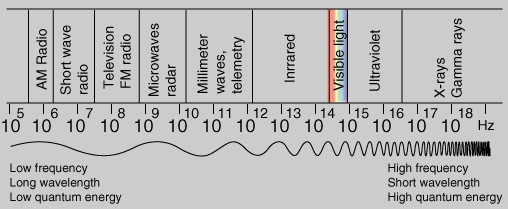
\includegraphics[scale=0.6]{waves}\caption{frequency scales}
\label{fig:waves to frequencies}
\end{figure}

\begin{itemize}
\item \href{http://www.grovemusic.com/shared/views/article.html?from=search&session_search_id=1013431856&session_name=f64e02b451f7a922&hitnum=1&section=music.00997&start=1&query=antheil&search_subview=search_subject}{Antheil} \textit{Ballet Mechanique} (1923-5)
\item \href{http://www.grovemusic.com/shared/views/article.html?from=search&session_search_id=1013432477&session_name=f64e02b451f7a922&hitnum=1&section=music.40105&start=1&query=satie&search_subview=search_subject}{Satie} \textit{Parade} (1917)
\item \href{http://www.grovemusic.com/shared/views/article.html?section=music.47335}{Respighi} \textit{Pines of Rome} (1924)
\item \href{http://www.grovemusic.com/shared/views/article.html?section=music.49908}{Cage} \textit{Imaginary Landscpes} (1939)
\item \href{http://www.grovemusic.com/shared/views/article.html?section=music.29042}{Var\`ese} \textit{Euqatorial} (1934), \textit{D\'eserts} (1950-54 ), \textit{Poem Electronique} (1958),
\end{itemize}


Futurists and Futurism:
\begin{itemize}
\item Filippo Tommaso Marinetti (1876-1944)
\item \href{http://www.grovemusic.com/shared/views/article.html?section=music.24174}{Luigi Russolo} (1885-1947)
\item \href{http://www.grovemusic.com/shared/views/article.html?from=search&session_search_id=1013432510&session_name=f64e02b451f7a922&hitnum=4&section=music.22259&start=1&query=marinetti&search_subview=search_subject}{Balilla Pratella} (1880-1965)
\end{itemize}

\begin{itemize}
\item Thaddeus Cahill (1867 - 1934) --- \href{http://www.grovemusic.com/shared/views/article.html?section=music.46183}{Telharmonium} 1897
\item \href{http://www.grovemusic.com/shared/views/article.html?section=music.45834}{Leon Theremin} (Lev Termen) (b St Petersburg, 15 Aug 1896; d Moscow, 3 Nov 1993)
\end{itemize}

\section{Pre-history 2}
\begin{itemize}
\item Electronic music developments in science and music
\item Schoenberg (1874-1951) - 5 orchestral pieces(1909) - III: Farben - Klangfarbenmelodie
\item Messiaen and the...Turanaglîla
\item Ondes Martenot - F\^te des Belles Eaux
\item Early Recording
\item Pierre Schaeffer in RTF - Cinq \'etudes de Bruits (1948) - \'Etudes aux objets (1959) - solfége
\item Jean Barraqu\'e - Etude (1953), Herbert Eimert + Robert Beyer - Klangstudie II (1952)
\item Stockhausen in RTF - Etude (1952)
\item Karlheinz Stockhausen in WDR - Electronishe Studies (1953, 1954), Gesang der J\"unglinge (1956), Kontakte (1960), Telemusik (1966), Hymnen (1966-7).
\end{itemize}

Schoenberg (writing to Mahler) ``..the possibility of creating a melody from one note played successively on different instruments''.

Messiaen (1908 - 1992): Oraison from 1937 is an extract from F\^ete des Belles Eaux. Commissioned and written for the world exposition in 1937

\begin{figure}[H]
\centering
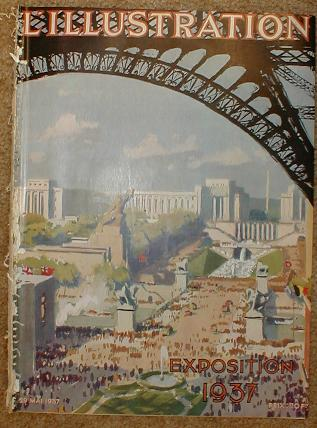
\includegraphics[scale=0.6]{illustration}\caption{world fair 1937}
\label{fig:worldfair}
\end{figure}

A Sons et lumi\'ere performance with fireworks and water jets. Twenty composers were commissioned. Many wrote orchestral works but Messiaen wrote for a sextet of Ondes Martenots. The music was amplified by loudspeakers placed buildings on the banks of the river Seine.

What does the ondes martenot do / look like?

\begin{figure}[H]
\centering
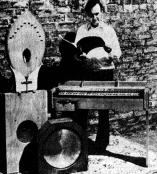
\includegraphics[scale=0.6]{mart}\caption{ondes martenot 1}
\label{fig:worldfair}
\end{figure}

\begin{figure}[H]
\centering
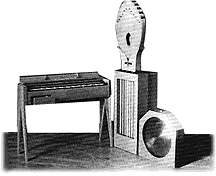
\includegraphics[scale=0.6]{martenot}\caption{ondes martenot 2}
\label{fig:worldfair}
\end{figure}

\subsection{Early Recording}
\begin{itemize}
\item Thomas Edison 1877, phonograph (hollow cylinder)
\item Emile Berliner 1887, flat disc gramophone
\item In 1925 Kurt Stille and partners licensed magnetic tape production to Ludwig Blattner and Kaul Bauer
\item In 1930 Marconi purchased Blattner's.
\item In Germany Fritz Pfleumer interested I.G.Farben in developing plastic backed tape (much lighter and safer) and Allgemeine Electrizitats Gesellsch\"ft (AEG) in developing machines. [by 1945 AEG had 15khz frequency response in magnetic tape at 30ips). Then the Minnesota Mining and Manufacture company developed a new tape (3M).
\end{itemize}

Sound in film - optical recordings had been around for some time and composers including the British composer Daphne Oram used this technique.

\section{Schaeffer (RTF) and Stockhausen (WDR)}

Schaeffer (1910-1995) and the GRM.

Studio d'Essai under German occupation 1942 / Club d'Essai in 1946. Groupe de Recherches Musicales (GRM) in 1958.

\begin{itemize}
\item Cinq \'etudes de Bruits (1948) - Concert de Bruits 1948
\item Symphonie pour un homme seul (1950) - with Pierre Henry (1927).
\item Etudes aux objets (1959)
\end{itemize}

\subsection{The Cologne studios}

Herbert Eimert (1897 - 1972), Robert Beyer (1901-1989) - Klangstudie II

\begin{enumerate}
\item demonstrate the analysis and synthesis of timbres:...
\item establish finely graduated scales between tone and noise
\item demonstrate the unity of musical time by creating graduated transitions between pitch and rhythm
\item use differentiated scales of loudness and reverberation to create a multi-layered spatial perspective.
\end{enumerate}

1948. Homer Dudley, from Bell Telephone Labs visited Werner Meyer Eppler.  Dudley had with him a new VOCODER – reactive filters on one side (reacting to sound A) that affect filters on the other side which filter Sound B. Robert Beyer was there from WDR. In 1950 they were joined by Herbert Eimert. Construction of the studio began in 1951/1952.  Bruno Maderna worked with Meyer-Eppler in Bonn (Institute of Phonetics, University of Bonn) and composed Musica su Due Dimensioni, (1952) for flute, percussion and tape which was performed that summer at Darmstadt to an audience that included PB, Gottfried Michael Koenig, Karel Goeyvaerts and KS.  The aesthetic was lead by Eimert who saw Elektronische Musik as an extension of serialism.

Serialism – understanding thereof.  Total serialism after Webern. 

KS began to work at WDR in May 1953.  \textit{Studie I} (1953) and \textit{Studie II} (1954) – see MUS201 / B+S course. Serial techniques to determine frequencies of sine waves.  Sounds being built up from first principles (Fourier after Helmholz).  Equipment resource consisted of a sine wave generator, a white noise generator, a melocord, and a monochord (a modified Trautonium built by Trautwein).  Most people (including KS) preferred to use the sine wave generator and a multitrack tape recorder.

\textit{Gesang der J\"unglinge} (1956) – mixture of natural and electronic but not a piece of musique concr\`ete by any means. (See B+S course).  A step away from serialism too with the warmth of natural colours and the pointillistic clouds.

1960 Stockhausen completed Kontakte.  Solo tape and tape + percussion + piano.  Moment Form.
 
During a visit to Japan he composed Telemusik (tele – all) – ring modulation.  1965, Solo for melody instrument with feeback.  1967 saw the completion of Hymnen.  Much intermodulation, ring modulation by high frequencies or rich modulation freqs that truly fused two signals – result often not an audible sign of either hence the mystical tag.  Stockhausen rubbished musique concr\`ete even then as `primitive collage'. 

He was director of WDR from 1962 to 1980.  Impressive list of equipment.  Composers attending during that time:

Gottfried Michael Koenig, Gyögy Ligeti, Mauricio Kagel, Konrad Boehmer, Mesias Maiguashca, Bernd Alois Zimmermann, York H\"oller, Roger Smalley, Jean-Claude Eloy, Tim Souster, Luc Ferrari, Iannis Xenakis.

\subsection{Var\`ese}
\begin{itemize}
\item 1920-21		Am\'eriques
\item 1921		Offrandes
\item 1922-23		Hyperprism
\item 1923		Octandre
\item 1923-25		Int\'egrales
\item 1926-27		Arcana
\item 1931		Ionisation
\item 1934		Ecuatorial
\item 1936		Density 21.5
\item 1950-54		D\'eserts
\item 1958		le Poem \'electronique
\item 1961		Nocturnal
\item 1965		Night (unfinished)
\end{itemize}

1916 Varèse said – ``Our musical alphabet must be enriched...we also need new instruments badly''.  The continuous flowing curve generated by the siren – (manual version of the oscillator). Var\`ese's ideas for an instrument similar to the Theremin was the Dynaphone.  Applications were made to the Guggenheim Foundation but were not successful. 

1954 – Var\`ese in Paris for tape parts for D\`eserts. 1957 – Philips Labs in Eindhoven, Holland for Poème Electronique.  There he met Xenakis. World's Fair in May 1958: Le Corbusier, (Charles-Edouard Jeanneret) (Le Corbusier) b1887 – 1965. Var\`ese and Xenakis. Music on a 3 track tape distributed over 425 loudspeakers.

\begin{itemize}
\item 1952 Konkrete Et\"ude (concrete music) - Stockhausen working with Schaeffer and studying with Messiaen
\item 1953 Elektronische Studie I
\item 1954 Electronische Studie II
\item 1955-6 Gesang der J\"nglinge
\item 1959-60 Kontakte (electronic and version for piano, percussion and electronics)
\item 1966 Telemusic (electronic music)
\item 1966 Hymnen (electronic and concrete music) - version with soloists - 1969 version with orchestra
\end{itemize}

\subsection{Japan}
1951 also in Japan: Tokyo
Joji Yuasa, Toru Takemistsu, Hiroyoshi Suzuki, Kazuo Fukushima founded Jikken Kobo (an experimental workshop). 1953 at NHK (Nippon Houso Kyokai / Japanese Broadcasting Corporation).  Joji Yuasa is perhaps best known out of the NHK crowd.

